%
% Tutorial -- Using Qucs in Textmode
%
% Copyright (C) 2013 Clemens Novak <clemens@familie-novak.net>
%
% Permission is granted to copy, distribute and/or modify this document
% under the terms of the GNU Free Documentation License, Version 1.1
% or any later version published by the Free Software Foundation.
%


\tutsection{Introduction}

Qucs consists of two parts: The simulator backend and a frontend, provding a GUI for drawing schematics, controlling simulation, and displaying the simulation results. The operation of the simulation backend is controlled via a text file (called \emph{netlist} in the following) which describes the circuit to be simulated and the simulation(s) to perform in a textual manner. The simulation backend outputs simulation data. This document describes the syntax of netlist files, shows how the netlists are actually used to control Qucs, and finally demonstrates how the simulation data can be visualized via GNU Octave.

Controlling Qucs via netlists and using a separate program for visualizing simulation data may seem complex at first glance; this approach, however, poses the advantage of allowing more flexible usage scenarios: The potentially cpu-consuming circuit simulation could be executed on a powerful (even remote) server, while the result visualization can be done locally on a different computer. By creating netlists via other programs / scripts, it is easy to setup batch simulations.


\tutsection{Outline}

After defining the prerequisites, Chaper \ref{chap:basics} presents a basic example netlist and shows how the simulation data can be visualized in Octave. Chapter \ref{chap:devices} describes the various devices and schematic elements provided by Qucs; Chapter \ref{chap:simulation} describes the simulation commands.


\tutsection{Basics}
\label{chap:basics}
\tutsection{Prerequisites}

Qucs installed \verb+qucsator+ command available

The m-files located under \verb+qucs/qucs/octave+.

\begin{verbatim}
Type:Name [node list] [parameters]
\end{verbatim}

Every schematic element has a type and is instantiated with a specific name.

\tutsection{Example}

In this chapter we will start with a simple example of performing an AC simulation of the circuit shown in Fig. \ref{fig:rc_ac_circuit}.

\begin{figure}[h]
\begin{center}
	\includegraphics[angle=0,width=0.4\linewidth]{rc_ac_circuit}
	\caption{Circuit}
	\label{fig:rc_ac_circuit}
\end{center}
\end{figure}

The texts in red denote the node names and can be chosen freely. The netlist corresponding to the circuit is shown below.

\begin{verbatim}
Vac:V1 in gnd U="1 V" f="1 kHz"
R:R1 out in R="1 kOhm"
C:C1 out gnd C="10 nF"
\end{verbatim}

It can be seen that the file is structured line-wise; every line instantiates one schematic element. The netlist instantiates

\begin{itemize}
\item a resistor R1 with resistance $R=1\text{k}\Omega$,
\item a capacitor C1 with capacity$C=10$nF, and
\item an AC source AC1 with "1"V peak-peak voltage(??) and a frequency of $1$kHz.
\end{itemize}

 Storing this netlist in a file \verb+rc_ac.net+ and feeding it into the simulator

\begin{verbatim}
qucsator < rc_ac.net
\end{verbatim}

yields the following result:

\begin{verbatim}
parsing netlist...
checking netlist...
checker error, no actions defined: nothing to do
\end{verbatim}

Qucs does not know what to do as we did not define any simulations to perform!

\tutsection{AC Sweep}

Deciding to perform an AC sweep, we add the another line to the netlist, yielding:

\begin{verbatim}
Vac:V1 in gnd U="1 V" f="1 kHz"
R:R1 out in R="1 kOhm"
C:C1 out gnd C="10 nF"

.AC:AC1 Type="log" Start="1 Hz" Stop="10 MHz" Points="300" Noise="no"
\end{verbatim}

Using this modified netlist with qucs starts an AC analysis of the circuit. The simulation data is written to stdout; for further processing we save the data in a file called \verb+rc_ac.dat+.

\begin{verbatim}
qucsator < rc_ac.net > rc_ac.dat
\end{verbatim}

The saved data from the simulation can be processed via Octave or Python; the next two subsections continue the example.

\begin{figure}[htb]
\begin{center}
  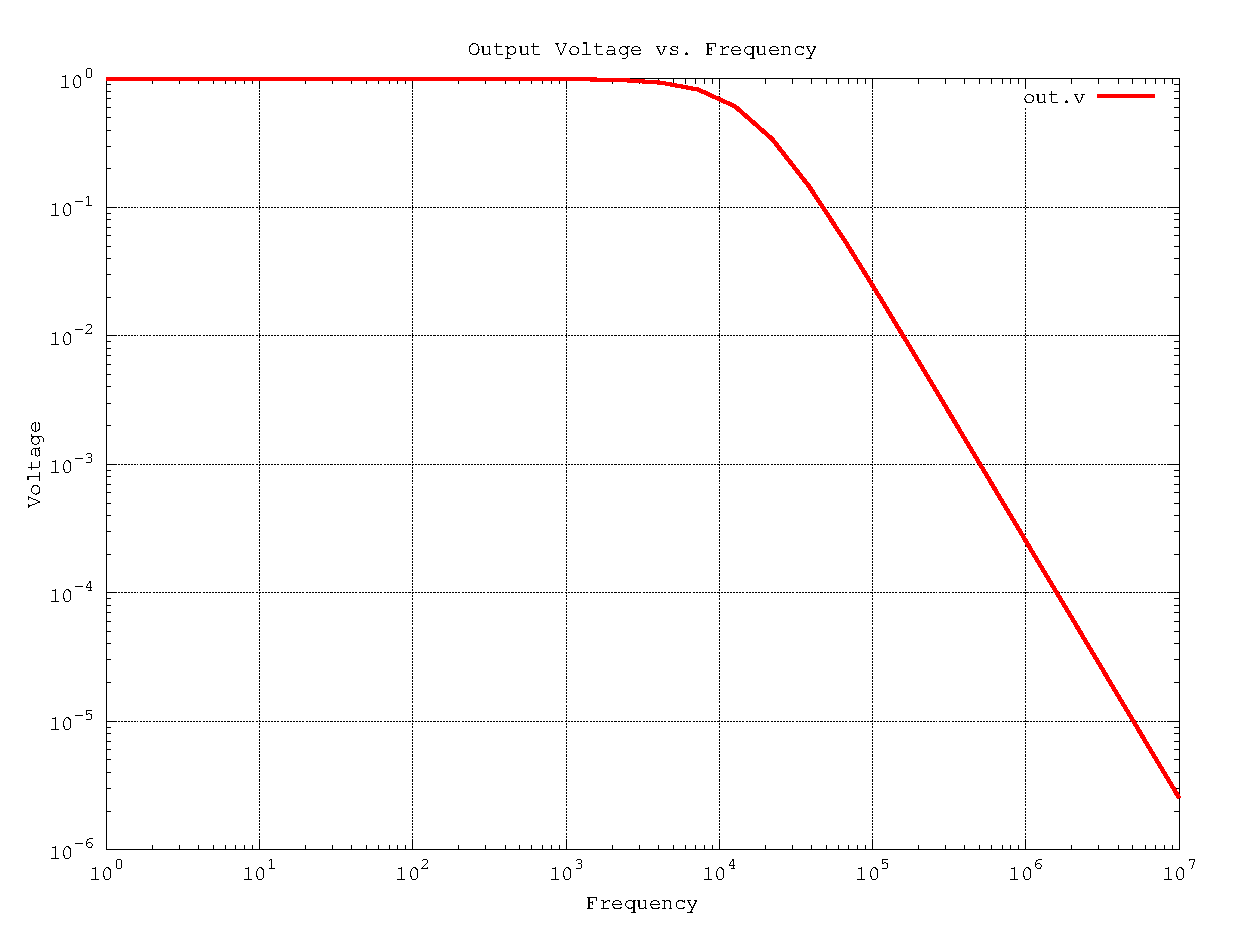
\includegraphics[angle=0,width=0.8\linewidth]{rc_ac}
  \caption{Simulation Result}
  \label{plot:rc_ac_octave}
\end{center}
\end{figure}


\tutsubsection{Analysis with Octave}



Starting GNU Octave and issuing the following commands

\begin{verbatim}
data=loadQucsDataSet('temp.dat')
loglog(data(1).data, data(3).data)
\end{verbatim}

produces a log-log plot of the output voltage versus the frequency. A slightly more polished plot is shown in Fig. \ref{plot:rc_ac_octave}.


\tutsubsection{Analysis with Python}

Similar to the octave scripts, Qucs provides a Python script which allows parsing of the generated simulation data file. The code example below shows how to load and parse the data file with Python. The plot using Matplotlib is shown in Fig. \ref{plot:rc_ac_python}.

% BUG: cant execute this from here!
\begin{verbatim}

import numpy as np
import matplotlib.pyplot as plt
import parse_result as pr

data = pr.parse_file('rc_ac.dat')

x = data['acfrequency']
y = np.abs(data['out.v'])

plt.loglog(x, y, '-r')
plt.grid()
plt.xlabel('Frequency')
plt.xlabel('Voltage')
plt.legend(['out.v'])
plt.show()
plt.savefig('rc_ac_python.eps') # save plot as eps file

\end{verbatim}


\begin{figure}[h]
\begin{center}
  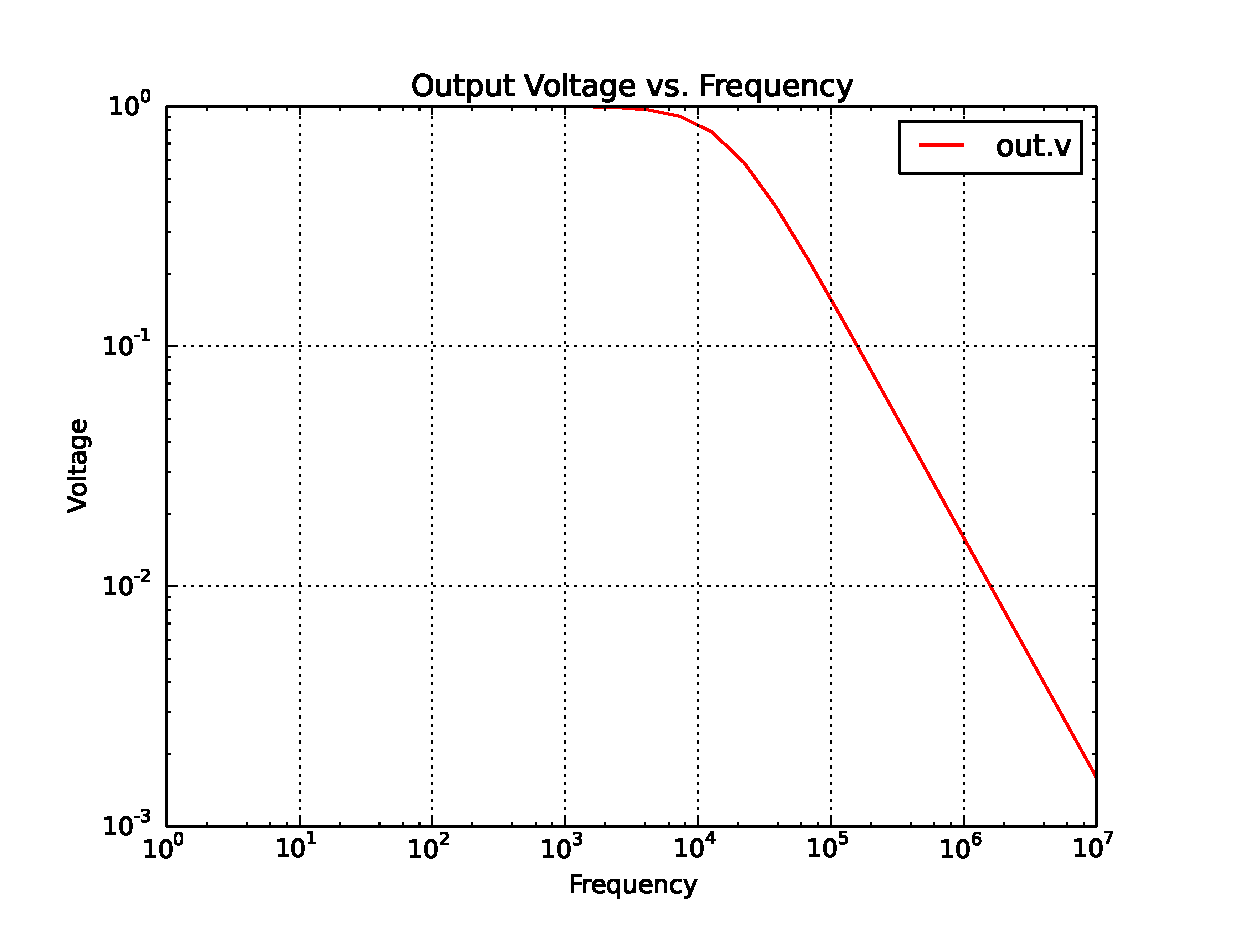
\includegraphics[angle=0,width=0.8\linewidth]{rc_ac_python}
  \caption{Simulation Result}
  \label{plot:rc_ac_python}
\end{center}
\end{figure}


\pagebreak

\paragraph{Nested Simulations.}Qucs allows for nested simulations; as an example we consider an AC analysis together with a parameter sweep. The AC analysis is set up as before, but in addition the value of the capacitor C1 is increased in $5$ steps from $10$nF to $100$nF. The netlist for this simulation is as follows.


\begin{verbatim}

Vac:V1 in gnd U="1 V" f="1 kHz"
R:R1 out in R="1 kOhm"
C:C1 out gnd C="Cx"

.SW:SW1 Sim="AC1" Type="lin" Param="Cx" Start="10 nF" Stop="100 nF" Points="5"

.AC:AC1 Start="1 Hz" Stop="10 MHz" Points="100" Type="log" Noise="no"

\end{verbatim}


The provided Python script can parse data files produced by such a nested simulation as well; in case of two nested simulations it returns not vectors, but matrices. The Python script below parses the simulation data file and plots the output voltage versus the frequency for two different capacitor values ($10$nF and $100$nF, respectively). The corresponding plot is shown in Fig. \ref{}.


\begin{verbatim}

import numpy as np
import matplotlib.pyplot as plt
import parse_result as pr

data = pr.parse_file('rc_ac_sweep.dat')

x = data['acfrequency']
y = np.abs(data['out.v'])
c = data['Cx']

plt.loglog(x,y[0,:],'-r')
plt.loglog(x,y[4,:],'-g')
plt.legend(['Cx=' + str(c[0]), 'Cx=' + str(c[4])])
plt.xlabel('Frequency')
plt.ylabel('Voltage')
plt.title('Output Voltage vs. Frequency')
plt.grid()
plt.savefig('rc_ac_sweep_python.eps')
plt.show()


\end{verbatim}


\begin{figure}[h]
\begin{center}
  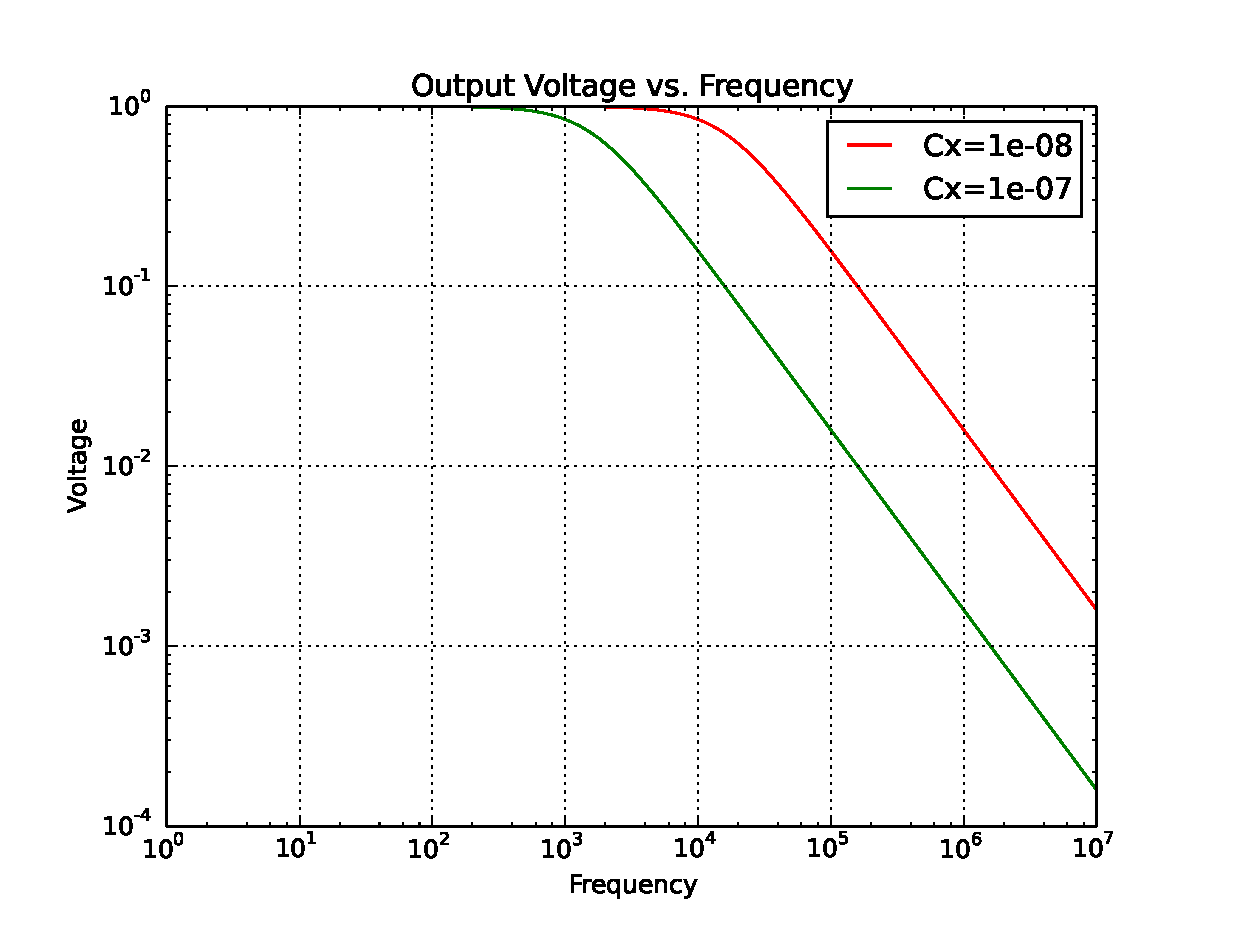
\includegraphics[angle=0,width=0.8\linewidth]{rc_ac_sweep_python}
  \caption{Simulation Result}
  \label{plot:rc_ac_python}
\end{center}
\end{figure}





\tutsection{Transient Simulation}

We can use almost the same circuit to perform a transient analysis

\begin{verbatim}
Vpulse:V1 in gnd U1=0 U2=1 T1="1 ns" T2="1 ms"
R:R1 out in R="1 kOhm"
C:C1 out gnd C="100 nF"

.TR:TR Type=lin Start="0" Stop="1.5 ms" Points="51"
\end{verbatim}

Here we have replaced the AC sourc with a voltage source generating pulses and told qucs to perform a transient analysis from $0$ to $1.5$ms. Storing the simulation results in a file and using octave to plot the results (analoguous to the previsou Subsection) yields the plot shown in Fig. \ref{plot:rc_ac_tr}-

\begin{figure}[h]
\begin{center}
  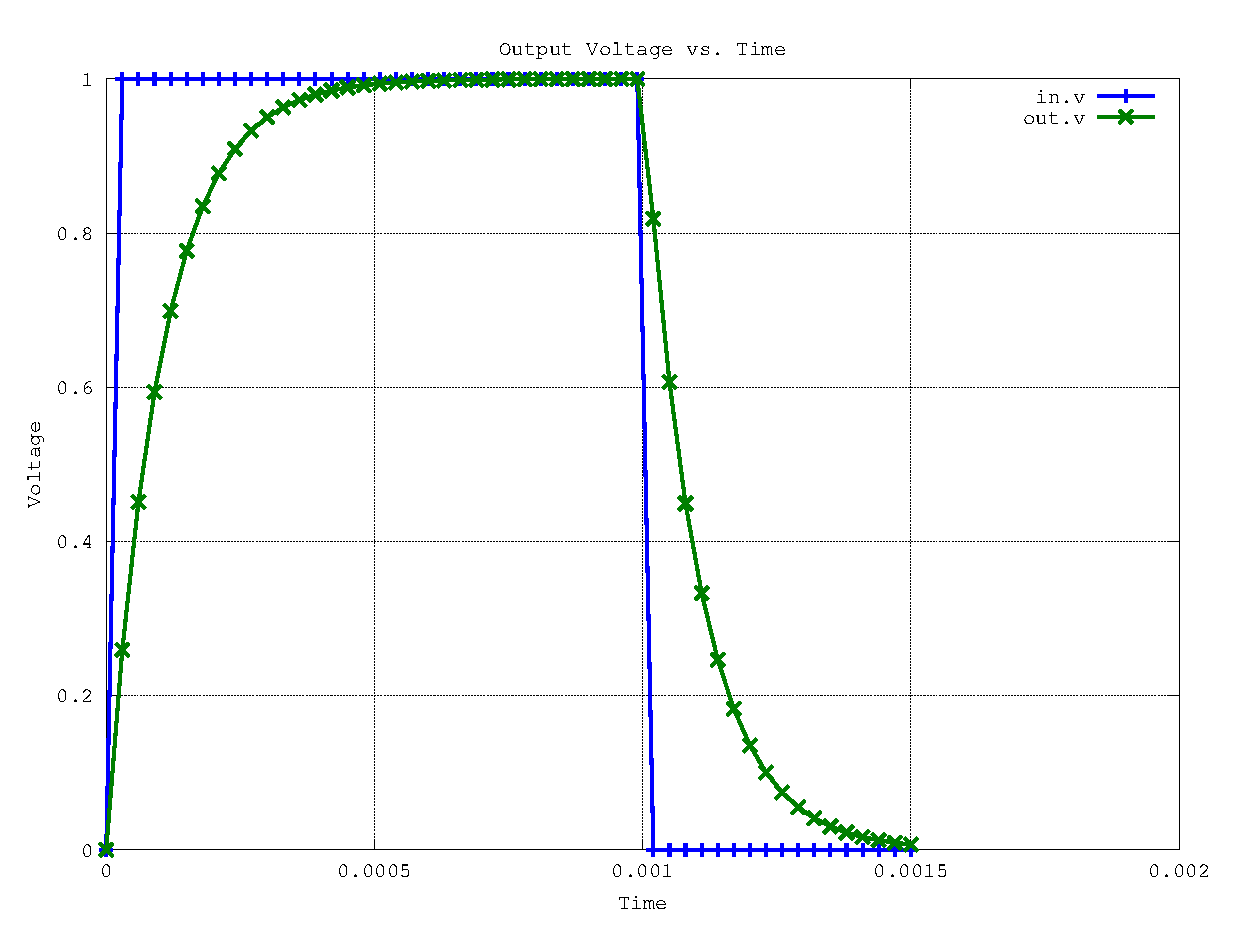
\includegraphics[angle=0,width=0.8\linewidth]{rc_ac_tr}
  \caption{Simulation Result}
  \label{plot:rc_ac_tr}
\end{center}
\end{figure}



\tutsection{Qucs Devices}
\label{chap:devices}

\tutsection{Passive Devices}

\subsection{Resistor}

\begin{verbatim}
R:Name Node1 Node2 [Parameters]
\end{verbatim}


\begin{tabular}{|l|p{0.5\linewidth}|l|l|}
\hline
Parameter & Name & Default & Value Mandatory \\
\hline
R & ohmic resistance in Ohms & n/a & yes \\
Temp & simulation temperature in degree Celsius & $26.85$ & no \\
Tc1 & first order temperature coefficient & $0.0$ & no \\
Tc2 & second order temperature coefficient & $0.0$ & no \\
Tnom & temperature at which parameters were extracted & $26.85$ & no \\
\hline
\end{tabular}


\subsection{Capacitor}

\begin{verbatim}
C:Name Node1 Node2 [Parameters]
\end{verbatim}


\begin{tabular}{|l|p{0.5\linewidth}|l|l|}
\hline
Parameter & Name & Default Value & Mandatory \\
\hline
C & capacitance in Farad & n/a & yes \\
V & initial voltage for transient simulation & n/a & no \\
\hline
\end{tabular}


\subsection{Inductor}

\begin{verbatim}
L:Name Node1 Node2 [Parameters]
\end{verbatim}


\begin{tabular}{|l|p{0.5\linewidth}|l|l|}
\hline
Parameter & Name & Default Value & Mandatory \\
\hline
L & inductance in Henry & n/a & yes \\
I & initial current for transient simulation & n/a & no \\
\hline
\end{tabular}


\tutsection{Nonlinear Components}

\subsection{Diode}

\begin{verbatim}
Diode:Name Cathode-Node Anode-Node [Parameters]
\end{verbatim}


\begin{tabular}{|l|p{0.5\linewidth}|l|l|}
\hline
Parameter & Name & Default Value & Mandatory \\
\hline
Is & saturation current & 1e-15 A & yes \\
N & emission coefficient & 1 & yes \\
Cj0 & zero-bias junction capacitance & 10 fF & yes \\
M & grading coefficient & 0.5 & yes \\
Vj & junction potential & 0.7 V & yes \\
Fc & forward-bias depletion capacitance coefficient & 0.5 & no \\
Cp & linear capacitance & 0.0 fF & no \\
Isr & recombination current parameter & 0.0 & no \\
Nr & emission coefficient for Isr & 2.0 & no \\
Rs & ohmic series resistance & 0.0 Ohm & no \\
Tt & transit time & 0.0 ps & no \\
Ikf & high-injection knee current (0=infinity) & 0 & no \\
Kf & flicker noise coefficient & 0.0 & no \\
Af & flicker noise exponent & 1.0 & no \\
Ffe & flicker noise frequency exponent & 1.0 & no \\
Bv & reverse breakdown voltage & 0 & no \\
Ibv & current at reverse breakdown voltage & 1 mA & no \\
Temp & simulation temperature in degree Celsius & 26.85 & no \\
Xti & saturation current temperature exponent & 3.0 & no \\
Eg & energy bandgap in eV & 1.11 & no \\
Tbv & Bv linear temperature coefficient & 0.0 & no \\
Trs & Rs linear temperature coefficient & 0.0 & no \\
Ttt1 & Tt linear temperature coefficient & 0.0 & no \\
Ttt2 & Tt quadratic temperature coefficient & 0.0 & no \\
Tm1 & M linear temperature coefficient & 0.0 & no \\
Tm2 & M quadratic temperature coefficient & 0.0 & no \\
Tnom & temperature at which parameters were extracted & 26.85 & no \\
Area & default area for diode & 1.0 & no \\
\hline
\end{tabular}


\subsection{Bipolar Junction Transistor with Substrate}

\begin{verbatim}
BJT:Name Base-Node Collector-Node Emitter-Node Substrate-Node [Parameters]
\end{verbatim}

\begin{tabular}{|l|p{0.5\linewidth}|l|l|}
\hline
Parameter & Name & Default & Value Mandatory \\
\hline
Type & Polarity [npn, pnp] & n/a & yes \\
Is & saturation current & 1e-16 & yes \\
Nf & forward emission coefficient & 1 & yes \\
Nr & reverse emission coefficient & 1 & yes \\
Ikf & high current corner for forward beta & 0 & yes \\
Ikr & high current corner for reverse beta & 0 & yes \\
Vaf & forward early voltage & 0 & yes \\
Var & reverse early voltage & 0 & yes \\
Ise & base-emitter leakage saturation current & 0 & yes \\
Ne & base-emitter leakage emission coefficient & 1.5 & yes \\
Isc & base-collector leakage saturation current & 0 & yes \\
Nc & base-collector leakage emission coefficient & 2 & yes \\
Bf & forward beta & 100 & yes \\
Br & reverse beta & 1 & yes \\
Rbm & minimum base resistance for high currents & 0 & yes \\
Irb & current for base resistance midpoint & 0 & yes \\
Rc & collector ohmic resistance & 0 & yes \\
Re & emitter ohmic resistance & 0 & yes \\
Rb & zero-bias base resistance (may be high-current dependent) & 0 & yes \\
Cje & base-emitter zero-bias depletion capacitance & 0 & yes \\
Vje & base-emitter junction built-in potential & 0.75 & yes \\
Mje & base-emitter junction exponential factor & 0.33 & yes \\
Cjc & base-collector zero-bias depletion capacitance & 0 & yes \\
Vjc & base-collector junction built-in potential & 0.75 & yes \\
Mjc & base-collector junction exponential factor & 0.33 & yes \\
Xcjc & fraction of Cjc that goes to internal base pin & 1.0 & yes \\
Cjs & zero-bias collector-substrate capacitance & 0 & yes \\
Vjs & substrate junction built-in potential & 0.75 & yes \\
Mjs & substrate junction exponential factor & 0 & yes \\
Fc & forward-bias depletion capacitance coefficient & 0.5 & yes \\
Tf & ideal forward transit time & 0.0 & yes \\
Xtf & coefficient of bias-dependence for Tf & 0.0 & yes \\
Vtf & voltage dependence of Tf on base-collector voltage & 0.0 & yes \\
Itf & high-current effect on Tf & 0.0 & yes \\
Tr & ideal reverse transit time & 0.0 & yes \\
Temp & simulation temperature in degree Celsius & 26.85 & no \\
Kf & flicker noise coefficient & 0.0 & no \\
Af & flicker noise exponent & 1.0 & no \\
Ffe & flicker noise frequency exponent & 1.0 & no \\
Kb & burst noise coefficient & 0.0 & no \\
Ab & burst noise exponent & 1.0 & no \\
Fb & burst noise corner frequency in Hertz & 1.0 & no \\
Ptf & excess phase in degrees & 0.0 & no \\
Xtb & temperature exponent for forward- and reverse beta & 0.0 & no \\
Xti & saturation current temperature exponent & 3.0 & no \\
Eg & energy bandgap in eV & 1.11 & no \\
Tnom & temperature at which parameters were extracted & 26.85 & no \\
Area & default area for bipolar transistor & 1.0 & no \\
\hline
\end{tabular}



\subsection{Diac}

\begin{verbatim}
Diac:Name Node1 Node2 [Parameters]
\end{verbatim}


\begin{tabular}{|l|p{0.5\linewidth}|l|l|}
\hline
Parameter & Name & Default Value & Mandatory \\
\hline
Vbo & (bidirectional) breakover voltage & 30 V & yes \\
Ibo & (bidirectional) breakover current & 50 uA & yes \\
Cj0 & parasitic capacitance & 10 pF & no \\
Is & saturation current & 1e-10 A & no \\
N & emission coefficient & 2 & no \\
Ri & intrinsic junction resistance & 10 Ohm & no \\
Temp & simulation temperature & 26.85 & no \\
\hline
\end{tabular}


\subsection{Silicon Controlled Rectifier (SCR)}

\begin{verbatim}
xxx:Name Node1 Node2 [Parameters]
\end{verbatim}


\begin{tabular}{|l|p{0.5\linewidth}|l|l|}
\hline
Parameter & Name & Default Value & Mandatory \\
\hline
Vbo & breakover voltage & 400 V & todo \\
Igt & gate trigger current & 50 uA & todo \\
Cj0 & parasitic capacitance & 10 pF & todo \\
Is & saturation current & 1e-10 A & todo \\
N & emission coefficient & 2 & todo \\
Ri & intrinsic junction resistance & 10 Ohm & todo \\
Rg & gate resistance & 5 Ohm & todo \\
Temp & simulation temperature & 26.85 & todo \\
\hline
\end{tabular}


\subsection{Triac (Bidirectional Thyristor)}

\begin{verbatim}
xxx:Name Node1 Node2 [Parameters]
\end{verbatim}


\begin{tabular}{|l|p{0.5\linewidth}|l|l|}
\hline
Parameter & Name & Default Value & Mandatory \\
\hline
Vbo & (bidirectional) breakover voltage & 400 V & todo \\
Igt & (bidirectional) gate trigger current & 50 uA & todo \\
Cj0 & parasitic capacitance & 10 pF & todo \\
Is & saturation current & 1e-10 A & todo \\
N & emission coefficient & 2 & todo \\
Ri & intrinsic junction resistance & 10 Ohm & todo \\
Rg & gate resistance & 5 Ohm & todo \\
Temp & simulation temperature & 26.85 & todo \\
\hline
\end{tabular}



\subsection{Resonance Tunnel Diode}

\begin{verbatim}
xxx:Name Node1 Node2 [Parameters]
\end{verbatim}


\begin{tabular}{|l|p{0.5\linewidth}|l|l|}
\hline
Parameter & Name & Default Value & Mandatory \\
\hline
Ip & peak current & 4 mA & todo \\
Iv & valley current & 0.6 mA & todo \\
Vv & valley voltage & 0.8 V & todo \\
Wr & resonance energy in Ws & 2.7e-20 & todo \\
eta & Fermi energy in Ws & 1e-20 & todo \\
dW & resonance width in Ws & 4.5e-21 & todo \\
Tmax & maximum of transmission & 0.95 & todo \\
de & fitting factor for electron density & 0.9 & todo \\
dv & fitting factor for voltage drop & 2.0 & todo \\
nv & fitting factor for diode current & 16 & todo \\
Cj0 & zero-bias depletion capacitance & 80 fF & todo \\
M & grading coefficient & 0.5 & todo \\
Vj & junction potential & 0.5 V & todo \\
te & life-time of electrons & 0.6 ps & todo \\
Temp & simulation temperature in degree Celsius & 26.85 & todo \\
Area & default area for diode & 1.0 & todo \\
\hline
\end{tabular}


\subsection{Junction Field-effect Transistor}

\begin{verbatim}
JFET:Name Gate-Node Drain-Node Source-Node [Parameters]
\end{verbatim}


\begin{tabular}{|l|p{0.5\linewidth}|l|l|}
\hline
Parameter & Name & Default Value & Mandatory \\
\hline
Type & polarity [nfet, pfet] & n/a & yes \\
Vt0 & threshold voltage & -2.0 V & yes \\
Beta & transconductance parameter & 1e-4 & yes \\
Lambda & channel-length modulation parameter & 0.0 & yes \\
Rd & parasitic drain resistance & 0.0 & yes \\
Rs & parasitic source resistance & 0.0 & yes \\
Is & gate-junction saturation current & 1e-14 & yes \\
N & gate-junction emission coefficient & 1.0 & yes \\
Isr & gate-junction recombination current parameter & 1e-14 & yes \\
Nr & Isr emission coefficient & 2.0 & yes \\
Cgs & zero-bias gate-source junction capacitance & 0.0 & yes \\
Cgd & zero-bias gate-drain junction capacitance & 0.0 & yes \\
Pb & gate-junction potential & 1.0 & yes \\
Fc & forward-bias junction capacitance coefficient & 0.5 & yes \\
M & gate P-N grading coefficient & 0.5 & yes \\
Kf & flicker noise coefficient & 0.0 & no \\
Af & flicker noise exponent & 1.0 & no \\
Ffe & flicker noise frequency exponent & 1.0 & no \\
Temp & simulation temperature in degree Celsius & 26.85 & no \\
Xti & saturation current temperature exponent & 3.0 & no \\
Vt0tc & Vt0 temperature coefficient & 0.0 & no \\
Betatce & Beta exponential temperature coefficient & 0.0 & no \\
Tnom & temperature at which parameters were extracted & 26.85 & no \\
Area & default area for JFET & 1.0 & no \\
\hline
\end{tabular}


\subsection{MOS field-effect transistor with substrate}

\begin{verbatim}
MOSFET:Name Gate-Node Drain-Node Source-Node Bulk-Nod[Parameters]
\end{verbatim}


\begin{tabular}{|l|p{0.5\linewidth}|l|l|}
\hline
Parameter & Name & Default Value & Mandatory \\
\hline
Type & polarity [nfet, pfet] & n/a & yes \\
Vt0 & zero-bias threshold voltage & 1.0 V & yes \\
Kp & transconductance coefficient in A/V$^2$ & 2e-5 & yes \\
Gamma & bulk threshold in sqrt(V) & yes \\
Phi & surface potential & 0.6 V & yes \\
Lambda & channel-length modulation parameter in 1/V & 0.0 & yes \\
Rd & drain ohmic resistance & 0.0 Ohm & no \\
Rs & source ohmic resistance & 0.0 Ohm & no \\
Rg & gate ohmic resistance & 0.0 Ohm & no \\
Is & bulk junction saturation current & 1e-14 A & yes \\
N & bulk junction emission coefficient & 1.0 & yes \\
W & channel width & 1 um & no \\
L & channel length & 1 um & no \\
Ld & lateral diffusion length & 0.0 & no \\
Tox & oxide thickness & 0.1 um & no \\
Cgso & gate-source overlap capacitance per meter of channel width in F/m & 0.0 & no \\
Cgdo & gate-drain overlap capacitance per meter of channel width in F/m & 0.0 & no \\
Cgbo & gate-bulk overlap capacitance per meter of channel length in F/m & 0.0 & no \\
Cbd & zero-bias bulk-drain junction capacitance & 0.0 F & no \\
Cbs & zero-bias bulk-source junction capacitance & 0.0 F & no \\
Pb & bulk junction potential & 0.8 V & no \\
Mj & bulk junction bottom grading coefficient & 0.5 & no \\
Fc & bulk junction forward-bias depletion capacitance coefficient & 0.5 & no \\
Cjsw & zero-bias bulk junction periphery capacitance per meter of junction perimeter in F/m & 0.0 & no \\
Mjsw & bulk junction periphery grading coefficient & 0.33 & no \\
Tt & bulk transit time & 0.0 ps & no \\
Nsub & substrate bulk doping density in 1/cm$^3$ & 0.0 & no \\
Nss & surface state density in 1/cm$^2$ & 0.0 & no \\
Tpg & gate material type: 0 = alumina; -1 = same as bulk; 1 = opposite to bulk & 0 & no \\
Uo & surface mobility in cm$^2$/Vs & 600.0 & no \\
Rsh & drain and source diffusion sheet resistance in Ohms/square & 0.0 & no \\
Nrd & number of equivalent drain squares & 1 & no \\
Nrs & number of equivalent source squares & 1 & no \\
Cj & zero-bias bulk junction bottom capacitance per square meter of junction area in F/m$^2$ & 0.0 & no \\
Js & bulk junction saturation current per square meter of junction area in A/m$^2$ & 0.0 & no \\
Ad & drain diffusion area in m$^2$ & 0.0 & no \\
As & source diffusion area in m$^2$ & 0.0 & no \\
Pd & drain junction perimeter & 0.0 m & no \\
Ps & source junction perimeter & 0.0 m & no \\
Kf & flicker noise coefficient & 0.0 & no \\
Af & flicker noise exponent & 1.0 & no \\
Ffe & flicker noise frequency exponent & 1.0 & no \\
Temp & simulation temperature in degree Celsius & 26.85 & no \\
Tnom & parameter measurement temperature & 26.85 & no \\
\hline
\end{tabular}


%% \tutsection{Verilog Devices}

%% EKV26MOS
%% HICUM Level 0 v1.12 verilog device
%% MESFET verilog device
%% NIGBT verilog device


\tutsection{Sources}


\subsection{DC Voltage Source}

\begin{verbatim}
V:Name Node1 Node2 [Parameters]
\end{verbatim}


\begin{tabular}{|l|p{0.5\linewidth}|l|l|}
\hline
Parameter & Name & Default Value & Mandatory \\
\hline
U & voltage in Volts & & yes \\
\hline
\end{tabular}


\subsection{AC Voltage Source}

\begin{verbatim}
Vac:Name Node1 Node2 [Parameters]
\end{verbatim}


\begin{tabular}{|l|p{0.5\linewidth}|l|l|}
\hline
Parameter & Name & Default Value & Mandatory \\
\hline
U & peak voltage in Volts & n/a & yes \\
f & frequency in Hertz & n/a & no \\
Phase & initial phase in degrees & 0 & no \\
Theta & damping factor (transient simulation only) & 0 & no \\
\hline
\end{tabular}



\subsection{Voltage Controlled Voltage Source}

\begin{verbatim}
VCVS:Name Node1 Node2 Node3 Node4 [Parameters]
\end{verbatim}

\verb+Node1+ is the input , \verb+Node2+ is the output, \verb+Node3+ is the ground for the input, and \verb+Node4+ is the ground for the output.


\begin{tabular}{|l|p{0.5\linewidth}|l|l|}
\hline
Parameter & Name & Default Value & Mandatory \\
\hline
G & forward transfer factor & 1.0 & todo \\
T & delay time & 0 & todo \\
\hline
\end{tabular}


\subsection{Voltage Controlled Current Source}

\begin{verbatim}
VCVS:Name Node1 Node2 Node3 Node4 [Parameters]
\end{verbatim}

\verb+Node1+ is the input , \verb+Node2+ is the output, \verb+Node3+ is the ground for the input, and \verb+Node4+ is the ground for the output.


\begin{tabular}{|l|p{0.5\linewidth}|l|l|}
\hline
Parameter & Name & Default Value & Mandatory \\
\hline
G & forward transconductance & 1.0 & todo \\
T & delay time & 0 & todo \\
\hline
\end{tabular}


\subsection{Current Controlled Voltage Source}

\begin{verbatim}
VCVS:Name Node1 Node2 Node3 Node4 [Parameters]
\end{verbatim}

\verb+Node1+ is the input , \verb+Node2+ is the output, \verb+Node3+ is the ground for the input, and \verb+Node4+ is the ground for the output.


\begin{tabular}{|l|p{0.5\linewidth}|l|l|}
\hline
Parameter & Name & Default Value & Mandatory \\
\hline
G & forward transfer factor & 1.0 & todo \\
T & delay time & 0 & todo \\
\hline
\end{tabular}


\subsection{Current Controlled Current Source}

\begin{verbatim}
VCVS:Name Node1 Node2 Node3 Node4 [Parameters]
\end{verbatim}

\verb+Node1+ is the input , \verb+Node2+ is the output, \verb+Node3+ is the ground for the input, and \verb+Node4+ is the ground for the output.


\begin{tabular}{|l|p{0.5\linewidth}|l|l|}
\hline
Parameter & Name & Default Value & Mandatory \\
\hline
G & forward transfer factor & 1.0 & todo \\
T & delay time & 0 & todo \\
\hline
\end{tabular}


\subsection{Voltage Pulse}

\begin{verbatim}
Vpulse:Name Node1 Node2 [Parameters]
\end{verbatim}


\begin{tabular}{|l|p{0.5\linewidth}|l|l|}
\hline
Parameter & Name & Default Value & Mandatory \\
\hline
U1& voltage before and after the pulse& 0 V& yes \\
U2& voltage of the pulse& 1 V& yes\\
T1& start time of the pulse& 0 & yes\\
T2& ending time of the pulse& 1 ms& yes\\
Tr& rise time of the leading edge& 1 ns & no\\
Tf& fall time of the trailing edge& 1 ns & no\\
\hline
\end{tabular}


\subsection{Current Pulse}

\begin{verbatim}
Ipulse:Name Node1 Node2 [Parameters]
\end{verbatim}


\begin{tabular}{|l|p{0.5\linewidth}|l|l|}
\hline
Parameter & Name & Default Value & Mandatory \\
\hline
I1& current before and after the pulse& 0 V& yes \\
I2& current of the pulse& 1 V& yes\\
T1& start time of the pulse& 0 & yes\\
T2& ending time of the pulse& 1 ms& yes\\
Tr& rise time of the leading edge& 1 ns & no\\
Tf& fall time of the trailing edge& 1 ns & no\\
\hline
\end{tabular}


\subsection{Rectangle Voltage}

\begin{verbatim}
Vrect:Name Node1 Node2 [Parameters]
\end{verbatim}


\begin{tabular}{|l|p{0.5\linewidth}|l|l|}
\hline
Parameter & Name & Default Value & Mandatory \\
\hline
U & voltage of high signal & 1 V & yes \\
TH & duration of high pulses & 1 ms & yes \\
TL & duration of low pulses & 1 ms & yes \\
Tr & rise time of the leading edge & 1 ns & todo \\
Tf & fall time of the leading edge & 1 ns & todo \\
Td & initial delay time & 0 ns & todo \\
\hline
\end{tabular}



\subsection{Rectangle Current}

\begin{verbatim}
Irect:Name Node1 Node2 [Parameters]
\end{verbatim}


\begin{tabular}{|l|p{0.5\linewidth}|l|l|}
\hline
Parameter & Name & Default Value & Mandatory \\
\hline
I & current at high pulse & 1 mA & yes \\
TH & duration of high pulses & 1 ms & yes \\
TL & duration of low pulses & 1 ms & yes \\
Tr & rise time of the leading edge & 1 ns & todo \\
Tf & fall time of the leading edge & 1 ns & todo \\
Td & initial delay time & 0 ns & todo \\
\hline
\end{tabular}


\subsection{Exponential Voltage Source}

\begin{verbatim}
Vexp:Name Node1 Node2 [Parameters]
\end{verbatim}


\begin{tabular}{|l|p{0.5\linewidth}|l|l|}
\hline
Parameter & Name & Default Value & Mandatory \\
\hline
U1 & voltage before rising edge & 0 V & todo \\
U2 & maximum voltage of the pulse & 1 V & todo \\
T1 & start time of the exponentially rising edge & 0 & todo \\
T2 & start of exponential decay & 1 ms & todo \\
Tr & rise time of the rising edge & 1 ns & todo \\
Tf & fall time of the falling edge & 1 ns & todo \\
\hline
\end{tabular}


\subsection{Exponential Current Source}

\begin{verbatim}
Vexp:Name Node1 Node2 [Parameters]
\end{verbatim}


\begin{tabular}{|l|p{0.5\linewidth}|l|l|}
\hline
Parameter & Name & Default Value & Mandatory \\
\hline
I1 & Current before rising edge & 0 V & todo \\
I2 & maximum current of the pulse & 1 A & todo \\
T1 & start time of the exponentially rising edge & 0 & todo \\
T2 & start of exponential decay & 1 ms & todo \\
Tr & rise time of the rising edge & 1 ns & todo \\
Tf & fall time of the falling edge & 1 ns & todo \\
\hline
\end{tabular}


\subsection{AC Voltage Source with Ammplitude Modulator}

\begin{verbatim}
AM_Mod:Name Node1 Node2 Node3 [Parameters]
\end{verbatim}

\verb+Node1+ is the modulated output, \verb+Node2+ is the common ground, and \verb+Node3+ is the modulation input.

\begin{tabular}{|l|p{0.5\linewidth}|l|l|}
\hline
Parameter & Name & Default Value & Mandatory \\
\hline
U & peak voltage in Volts & 1 V & todo \\
f & frequency in Hertz & 1 GHz & todo \\
Phase & initial phase in degrees & 0 & todo \\
m & modulation level & 1.0 & todo \\
\hline
\end{tabular}



\subsection{AC Voltage Source with Ammplitude Modulator}

\begin{verbatim}
AM_Mod:Name Node1 Node2 Node3 [Parameters]
\end{verbatim}

\verb+Node1+ is the modulated output, \verb+Node2+ is the common ground, and \verb+Node3+ is the modulation input.

\begin{tabular}{|l|p{0.5\linewidth}|l|l|}
\hline
Parameter & Name & Default Value & Mandatory \\
\hline
U & peak voltage in Volts & 1 V & todo \\
f & frequency in Hertz & 1 GHz & todo \\
Phase & initial phase in degrees & 0 & todo \\
m & modulation level & 1.0 & todo \\
\hline
\end{tabular}



\subsection{AC Voltage Source with Phase Modulator}

\begin{verbatim}
PM_Mod:Name Node1 Node2 Node3 [Parameters]
\end{verbatim}

\verb+Node1+ is the modulated output, \verb+Node2+ is the common ground, and \verb+Node3+ is the modulation input.

\begin{tabular}{|l|p{0.5\linewidth}|l|l|}
\hline
Parameter & Name & Default Value & Mandatory \\
\hline
U & peak voltage in Volts & 1 V & todo \\
f & frequency in Hertz & 1 GHz & todo \\
Phase & initial phase in degrees & 0 & todo \\
M & modulation index & 1.0 & todo \\
\hline
\end{tabular}



% & & & \\

\tutsection{Simulation Commands}
\label{chap:simulation}


\tutsection{DC Simulation}


\begin{verbatim}
.DC:Name [Parameters]
\end{verbatim}


\begin{tabular}{|l|p{0.5\linewidth}|l|l|}
\hline
Parameter & Name & Default Value & Mandatory \\
\hline
Temp & simulation temperature in degree Celsius& $26.85$ & no \\
reltol & relative tolerance for convergence & 0.001 & no \\
absol & absolute tolerance for currents & 1 pA & no \\
vntol & absolute tolerance for voltages & 1 uV & no \\
saveOPs & put operating points into dataset [yes,no]& & no \\
MaxIter & maximum number of iterations until error & 150 & no \\
saveAll & save subcircuit nodes into dataset [yes,no]& no & no\\
convHelper & preferred convergence algorithm [none, gMinStepping, SteepestDescent, LineSearch, Attenuation, SourceStepping]& none & \\
Solver & method for solving the circuit matrix [CroutLU, DoolittleLU, HouseholderQR, HouseholderLQ, GolubSVD] & CroutLU & no \\
\hline
\end{tabular}


\tutsection{AC Simulation}


\begin{verbatim}
.AC:Name [Parameters]
\end{verbatim}


\begin{tabular}{|l|p{0.5\linewidth}|l|l|}
\hline
Parameter & Name & Default Value & Mandatory \\
\hline
Type & sweep type [lin,log,list,const] & n/a & yes \\
Start & start frequency in Hertz & n/a & yes \\
Stop & stop frequency in Hertz & n/a & yes \\
Points & number of simulation steps & n/a & yes \\
Noise & calculate noise voltages & no & no \\
\hline
\end{tabular}



\tutsection{Parameter Sweep}


\begin{verbatim}
.SW:Name [Parameters]
\end{verbatim}


\begin{tabular}{|l|p{0.5\linewidth}|l|l|}
\hline
Parameter & Name & Default Value & Mandatory \\
\hline
Sim & simulation to perform parameter sweep on & n/a & yes \\
Type & sweep type [lin,log,list,const] & n/a & yes \\
Param & parameter to sweep & n/a & yes \\
Stop & start value for sweep & n/a & yes \\
Start & stop value for sweep & n/a & yes \\
\hline
\end{tabular}



\tutsection{Transient Simulation}


\begin{verbatim}
.TR:Name [Parameters]
\end{verbatim}


\begin{tabular}{|l|p{0.5\linewidth}|l|l|}
\hline
Parameter & Name & Default Value & Mandatory \\
\hline
Type & sweep type [lin,log,list,const] & todo & todo \\
Start & start time in seconds & todo & todo \\
Stop & stop time in seconds & todo & todo \\
Points & number of simulation time steps & 11(todo) & todo \\
IntegrationMethod & integration method [Euler, Trapezoidal, Gear, AdamsMoulton] & Trapezoidal & todo \\
Order & order of integration method & 2 & todo \\
InitialStep & initial step size in seconds & 1 ns (todo) & todo \\
MinStep & minimum step size in seconds & 1e-16 & todo \\
MaxIter & maximum number of iterations until error & 150 & todo \\
reltol & relative tolerance for convergence & 0.001 & todo \\
abstol & absolute tolerance for currents & 1 pA & todo \\
vntol & absolute tolerance for voltages & 1 uV & todo \\
Temp & simulation temperature in degree Celsius & 26.85 & todo \\
LTEreltol & relative tolerance of local truncation error & 1e-3 & todo \\
LTEabstol & absolute tolerance of local truncation error & 1e-6 & todo \\
LTEfactor & overestimation of local truncation error & 1 & todo \\
Solver & method for solving the circuit matrix [CroutLU, DoolittleLU, HouseholderQR, HouseholderLQ, GolubSVD] & CroutLU & todo \\
relaxTSR & relax time step raster [no, yes] & yes & todo \\
initialDC & perform an initial DC analysis [yes, no] & yes & todo \\
MaxStep & maximum step size in seconds & 0 & todo \\
\hline
\end{tabular}


\tutsection{S Parameter Simulation}

\begin{verbatim}
xxx:Name Node1 Node2 [Parameters]
\end{verbatim}


\begin{tabular}{|l|p{0.5\linewidth}|l|l|}
\hline
Parameter & Name & Default Value & Mandatory \\
\hline
Type & sweep type [lin,log,list,const] & todo & todo \\
Start & start frequency in Hertz & 1 GHz & todo \\
Stop & stop frequency in Hertz & 10 GHz & todo \\
Points & number of simulation steps & 19 & todo \\
Noise & calculate noise parameters & no & todo \\
NoiseIP & input port for noise figure & 1 & todo \\
NoiseOP & output port for noise figure & 2 & todo \\
saveCVs & put characteristic values into dataset [yes,no] & no & todo \\
saveAll & save subcircuit characteristic values into dataset [yes,no] & no & todo \\
\hline
\end{tabular}

\subsection{xxx}

\begin{verbatim}
xxx:Name Node1 Node2 [Parameters]
\end{verbatim}


\begin{tabular}{|l|p{0.5\linewidth}|l|l|}
\hline
Parameter & Name & Default Value & Mandatory \\
\hline
L & inductance in Henry & n/a & yes \\
\hline
\end{tabular}




\subsection{Silicon Controlled Rectifier (SCR)}

\begin{verbatim}
xxx:Name Node1 Node2 [Parameters]
\end{verbatim}


\begin{tabular}{|l|p{0.5\linewidth}|l|l|}
\hline
Parameter & Name & Default Value & Mandatory \\
\hline
Vbo & breakover voltage & 400 V & todo \\
Igt & gate trigger current & 50 uA & todo \\
Cj0 & parasitic capacitance & 10 pF & todo \\
Is & saturation current & 1e-10 A & todo \\
N & emission coefficient & 2 & todo \\
Ri & intrinsic junction resistance & 10 Ohm & todo \\
Rg & gate resistance & 5 Ohm & todo \\
Temp & simulation temperature & 26.85 & todo \\
\hline
\end{tabular}


\subsection{Triac (Bidirectional Thyristor)}

\begin{verbatim}
xxx:Name Node1 Node2 [Parameters]
\end{verbatim}


\begin{tabular}{|l|p{0.5\linewidth}|l|l|}
\hline
Parameter & Name & Default Value & Mandatory \\
\hline
Vbo & (bidirectional) breakover voltage & 400 V & todo \\
Igt & (bidirectional) gate trigger current & 50 uA & todo \\
Cj0 & parasitic capacitance & 10 pF & todo \\
Is & saturation current & 1e-10 A & todo \\
N & emission coefficient & 2 & todo \\
Ri & intrinsic junction resistance & 10 Ohm & todo \\
Rg & gate resistance & 5 Ohm & todo \\
Temp & simulation temperature & 26.85 & todo \\
\hline
\end{tabular}



\subsection{Resonance Tunnel Diode}

\begin{verbatim}
xxx:Name Node1 Node2 [Parameters]
\end{verbatim}


\begin{tabular}{|l|p{0.5\linewidth}|l|l|}
\hline
Parameter & Name & Default Value & Mandatory \\
\hline
Ip & peak current & 4 mA & todo \\
Iv & valley current & 0.6 mA & todo \\
Vv & valley voltage & 0.8 V & todo \\
Wr & resonance energy in Ws & 2.7e-20 & todo \\
eta & Fermi energy in Ws & 1e-20 & todo \\
dW & resonance width in Ws & 4.5e-21 & todo \\
Tmax & maximum of transmission & 0.95 & todo \\
de & fitting factor for electron density & 0.9 & todo \\
dv & fitting factor for voltage drop & 2.0 & todo \\
nv & fitting factor for diode current & 16 & todo \\
Cj0 & zero-bias depletion capacitance & 80 fF & todo \\
M & grading coefficient & 0.5 & todo \\
Vj & junction potential & 0.5 V & todo \\
te & life-time of electrons & 0.6 ps & todo \\
Temp & simulation temperature in degree Celsius & 26.85 & todo \\
Area & default area for diode & 1.0 & todo \\
\hline
\end{tabular}


%% \begin{tabular}{|l|p{0.5\linewidth}|l|l|}
%% \hline
%% Parameter & Name & Default Value & Mandatory \\
%% \hline
%% L & inductance in Henry & n/a & yes \\
%% \hline
%% \end{tabular}

